\documentclass{article}[fleqn]

\usepackage{fancyhdr}
\usepackage{extramarks}
\usepackage{amsmath}
\usepackage{amsthm}
\usepackage{amsfonts}
\usepackage{tikz}
\usepackage[edges]{forest}
\usepackage[plain]{algorithm}
\usepackage{algpseudocode}
\usepackage[utf8]{inputenc} % Umlaute
\usepackage{ulem} % underline with wordwrap \uline
\usepackage{etoolbox}
\AtBeginEnvironment{align}{\setcounter{equation}{0}}
\usepackage{prooftrees} 
\usepackage{tikz}
\usepackage{tikz-qtree}
%\usetikzlibrary{graphdrawing.trees}
\usepackage{tabularx, caption}
\usepackage{ragged2e}
\usepackage{tcolorbox}
\usepackage{pifont}
\usepackage{enumitem}
\newcommand{\cmark}{\ding{51}}
\usepackage{subcaption}
\renewcommand{\labelitemi}{$\circ$}

\usetikzlibrary{automata,positioning}

% ///////////////////////
% Basic Document Settings
% ///////////////////////

\topmargin=-0.45in
\evensidemargin=0in
\oddsidemargin=0in
\textwidth=6.5in
\textheight=9.0in
\headsep=0.25in

\linespread{1.1}

% Tablestuff
\def\arraystretch{1.5}
\newcolumntype{L}{>{\RaggedRight} X}

\pagestyle{fancy}
\lhead{\hmwkAuthorName, \hmwkMatrikel}
\chead{\hmwkClass: \hmwkTitle}
\rhead{\firstxmark}
\lfoot{\lastxmark}
\cfoot{\thepage}

\renewcommand\headrulewidth{0.4pt}
\renewcommand\footrulewidth{0.4pt}

\newcommand{\splitter}{\noindent\rule{\textwidth}{1pt}}

\setlength{\parskip}{\baselineskip}%
\setlength\parindent{0pt}

% Tcolorbox
\definecolor{frame}{RGB}{214, 214, 239}
\definecolor{back}{RGB}{234, 234, 247}
\tcbset{colback=back,colframe=frame,coltitle=blue,boxrule=0mm,boxsep=6pt,left=2pt,right=2pt,top=0pt,bottom=0pt}

% ///////////////////////
% Create Problem Sections
% ///////////////////////

\newcommand{\enterProblemHeader}[1]{
    \nobreak\extramarks{}{Continuation on the next page\ldots}\nobreak{}
    \nobreak\extramarks{Exercise \arabic{#1} (Continuation)}{Continuation on the next page\ldots}\nobreak{}
}

\newcommand{\exitProblemHeader}[1]{
    \nobreak\extramarks{Exercise \arabic{#1} (Continuation)}{Continuation on the next page\ldots}\nobreak{}
    \stepcounter{#1}
    \nobreak\extramarks{Exercise \arabic{#1}}{}\nobreak{}
}



\setcounter{secnumdepth}{0}
\newcounter{partCounter}
\newcounter{homeworkProblemCounter}

% ///////////////////////////////////
% Initialize the problem counter here
% ///////////////////////////////////
\setcounter{homeworkProblemCounter}{1}
\nobreak\extramarks{Exercise \arabic{homeworkProblemCounter}}{}\nobreak{}

% ////////////////////////////
% Homework Problem Environment
% ////////////////////////////
% This environment takes an optional argument. When given, it will adjust the
% problem counter. This is useful for when the problems given for your
% assignment aren't sequential. See the last 3 problems of this template for an
% example.
%
\newenvironment{homeworkProblem}[1][-1]{
    \ifnum#1>0
        \setcounter{homeworkProblemCounter}{#1}
    \fi
    \section{Exercise \arabic{homeworkProblemCounter}}
    \setcounter{partCounter}{1}
    \enterProblemHeader{homeworkProblemCounter}
}{
    \exitProblemHeader{homeworkProblemCounter}
}

% ////////////////
% Homework Details
%   - Title
%   - Due date
%   - Class
%   - Section/Time
%   - Instructor
%   - Author
% ////////////////

\newcommand{\hmwkTitle}{Exercise 2}
\newcommand{\hmwkDueDate}{09.05.2019}
\newcommand{\hmwkClass}{EKI}
\newcommand{\hmwkClassTime}{}
\newcommand{\hmwkClassInstructor}{}
\newcommand{\hmwkAuthorName}{STUDENT NAME}
\newcommand{\hmwkMatrikel}{MAT NUMBER}

% //////////
% Title Page
% //////////

\title{
    \vspace{2in}
    \textmd{\textbf{\hmwkClass:\ \hmwkTitle}}\\
    \normalsize\vspace{0.1in}\small{\hmwkDueDate}\\
    \vspace{0.1in}\large{\textit{\hmwkClassInstructor\ \hmwkClassTime}}
    \vspace{3in}
}

\author{\textbf{\hmwkAuthorName, \hmwkMatrikel}}
\date{}

\renewcommand{\part}[1]{\textbf{
    \\[\baselineskip]
    \large Part
    \alph{partCounter}
    }\stepcounter{partCounter}}

% ///////////////////////
% Various Helper Commands
% ///////////////////////

% Useful for algorithms
\newcommand{\alg}[1]{\textsc{\bfseries \footnotesize #1}}

% For derivatives
\newcommand{\deriv}[1]{\frac{\mathrm{d}}{\mathrm{d}x} (#1)}

% For partial derivatives
\newcommand{\pderiv}[2]{\frac{\partial}{\partial #1} (#2)}

% Integral dx
\newcommand{\dx}{\mathrm{d}x}

% Alias for the Solution section header
\newcommand{\solution}{\textbf{\large \\Solution}}

% Probability commands: Expectation, Variance, Covariance, Bias
\newcommand{\calI}{{\cal I}}
\newcommand{\calM}{{\cal M}}
\newcommand{\eq}{\leftrightarrow}

\begin{document}

\maketitle
\pagebreak

% ///////////////////////
% Regular Problem example
% ///////////////////////
%\twocolumn
\begin{homeworkProblem}
    You and a group of friends decide to estimate how much effort you need to put into the Introduction to Artificial Intelligence course to successfully pass the exam.
        
    You first decide what data is relevant for your decision and after some discussion, you settle for the attributes $H$ (how many hours the student approximately spent studying and preparing for the exam) with the domain $V (H) = {10,30,50}$, $E$ (whether the student participated in the exercise part) with the domain $V (E) = {\top,\bot}$, $T$ (whether the student clarified open questions with the tutors) with the domain $V (T) = {\top,\bot}$. Content with your rather simplistic model, you ask some older colleagues who have already taken the course for their experience and collect the following data:

    \begin{table}[ht]
        \setlength\extrarowheight{-3pt}
        \centering
        \begin{tabular}{r||c|c|c||c}
            Sample & $H$ & $E$ & $T$ & Passed? \\
            \hline \hline
            1 & 10 & $\top$ & $\top$ & $F$\\
            2 & 30 & $\top$ & $\top$ & $T$\\
            3 & 50 & $\top$ & $\top$ & $T$\\
            4 & 10 & $\top$ & $\bot$ & $F$\\
            5 & 30 & $\top$ & $\bot$ & $F$\\
            6 & 50 & $\top$ & $\bot$ & $T$\\
            7 & 10 & $\bot$ & $\bot$ & $F$\\
            8 & 30 & $\bot$ & $\bot$ & $F$\\
            9 & 50 & $\bot$ & $\bot$ & $T$
        \end{tabular}
    \end{table}

    Use the gathered data to construct a decision tree capable of predicting whether a given student will pass their exam, given the values of the attributes you chose. In each step of the construction, choose the attribute that maximizes the information gain, as shown in the lecture.

    \solution{}

\end{homeworkProblem}

\begin{homeworkProblem}

     Construct another decision tree for Exercise 2.1, this time choosing the attribute that maximizes the \textit{relative information} gain, i.e. the ratio between the gain of the attribute and its own intrinsic information.

     \[GainR(A) = \frac{Gain(A)}{H(A)}\]

     and
     \[H(A):= \sum_{a\in V(A)} \frac{|E_a|}{V} \text{log}_2 \frac{V}{|E_a|}\]

     where $V(A)$ denotes the domain of the attribute $A$, and $|E_a|$ is the number of all samples which have the value $a$ of the attribute $A$. Furthermore, we define $V := \sum_{a\in V(A)} |E_a|$ to be the size of the set of all samples.

    \solution{}

\end{homeworkProblem}

\begin{homeworkProblem}
     In this exercise we explore some of the problems with decision trees and the ways of dealing with them:

    \begin{enumerate}[label=(\alph*)]
        \item Compute the relative information gain for an attribute $A$ which takes a different value for each example (Assume that you are given $2n$ examples, which are distributed evenly between two classes). Can you spot the advantage of using the relative information gain rather than the regular information gain rule? Compare with an attribute $B$ which splits the example set in exactly two halves with the correct classification.
        \item Suppose that you’re collecting data for a decision tree. The first two examples you collect have the exact same value for each of the attributes you picked, but their classification is different. You stop collecting further data and ponder the implications of the situation that occurred. Discuss briefly the answers to the following questions:
        \begin{itemize}
            \item What could be the cause for such a situation?
            \item What would the decision tree learning algorithm discussed in the lecture do in this case?
            \item What could you do to avoid the problem that arises?
        \end{itemize}
    \end{enumerate}
    \solution{}

\end{homeworkProblem}

\begin{homeworkProblem}
    Consider a neural network with six nodes of the following form:
    \begin{figure}[h]
        \centering
        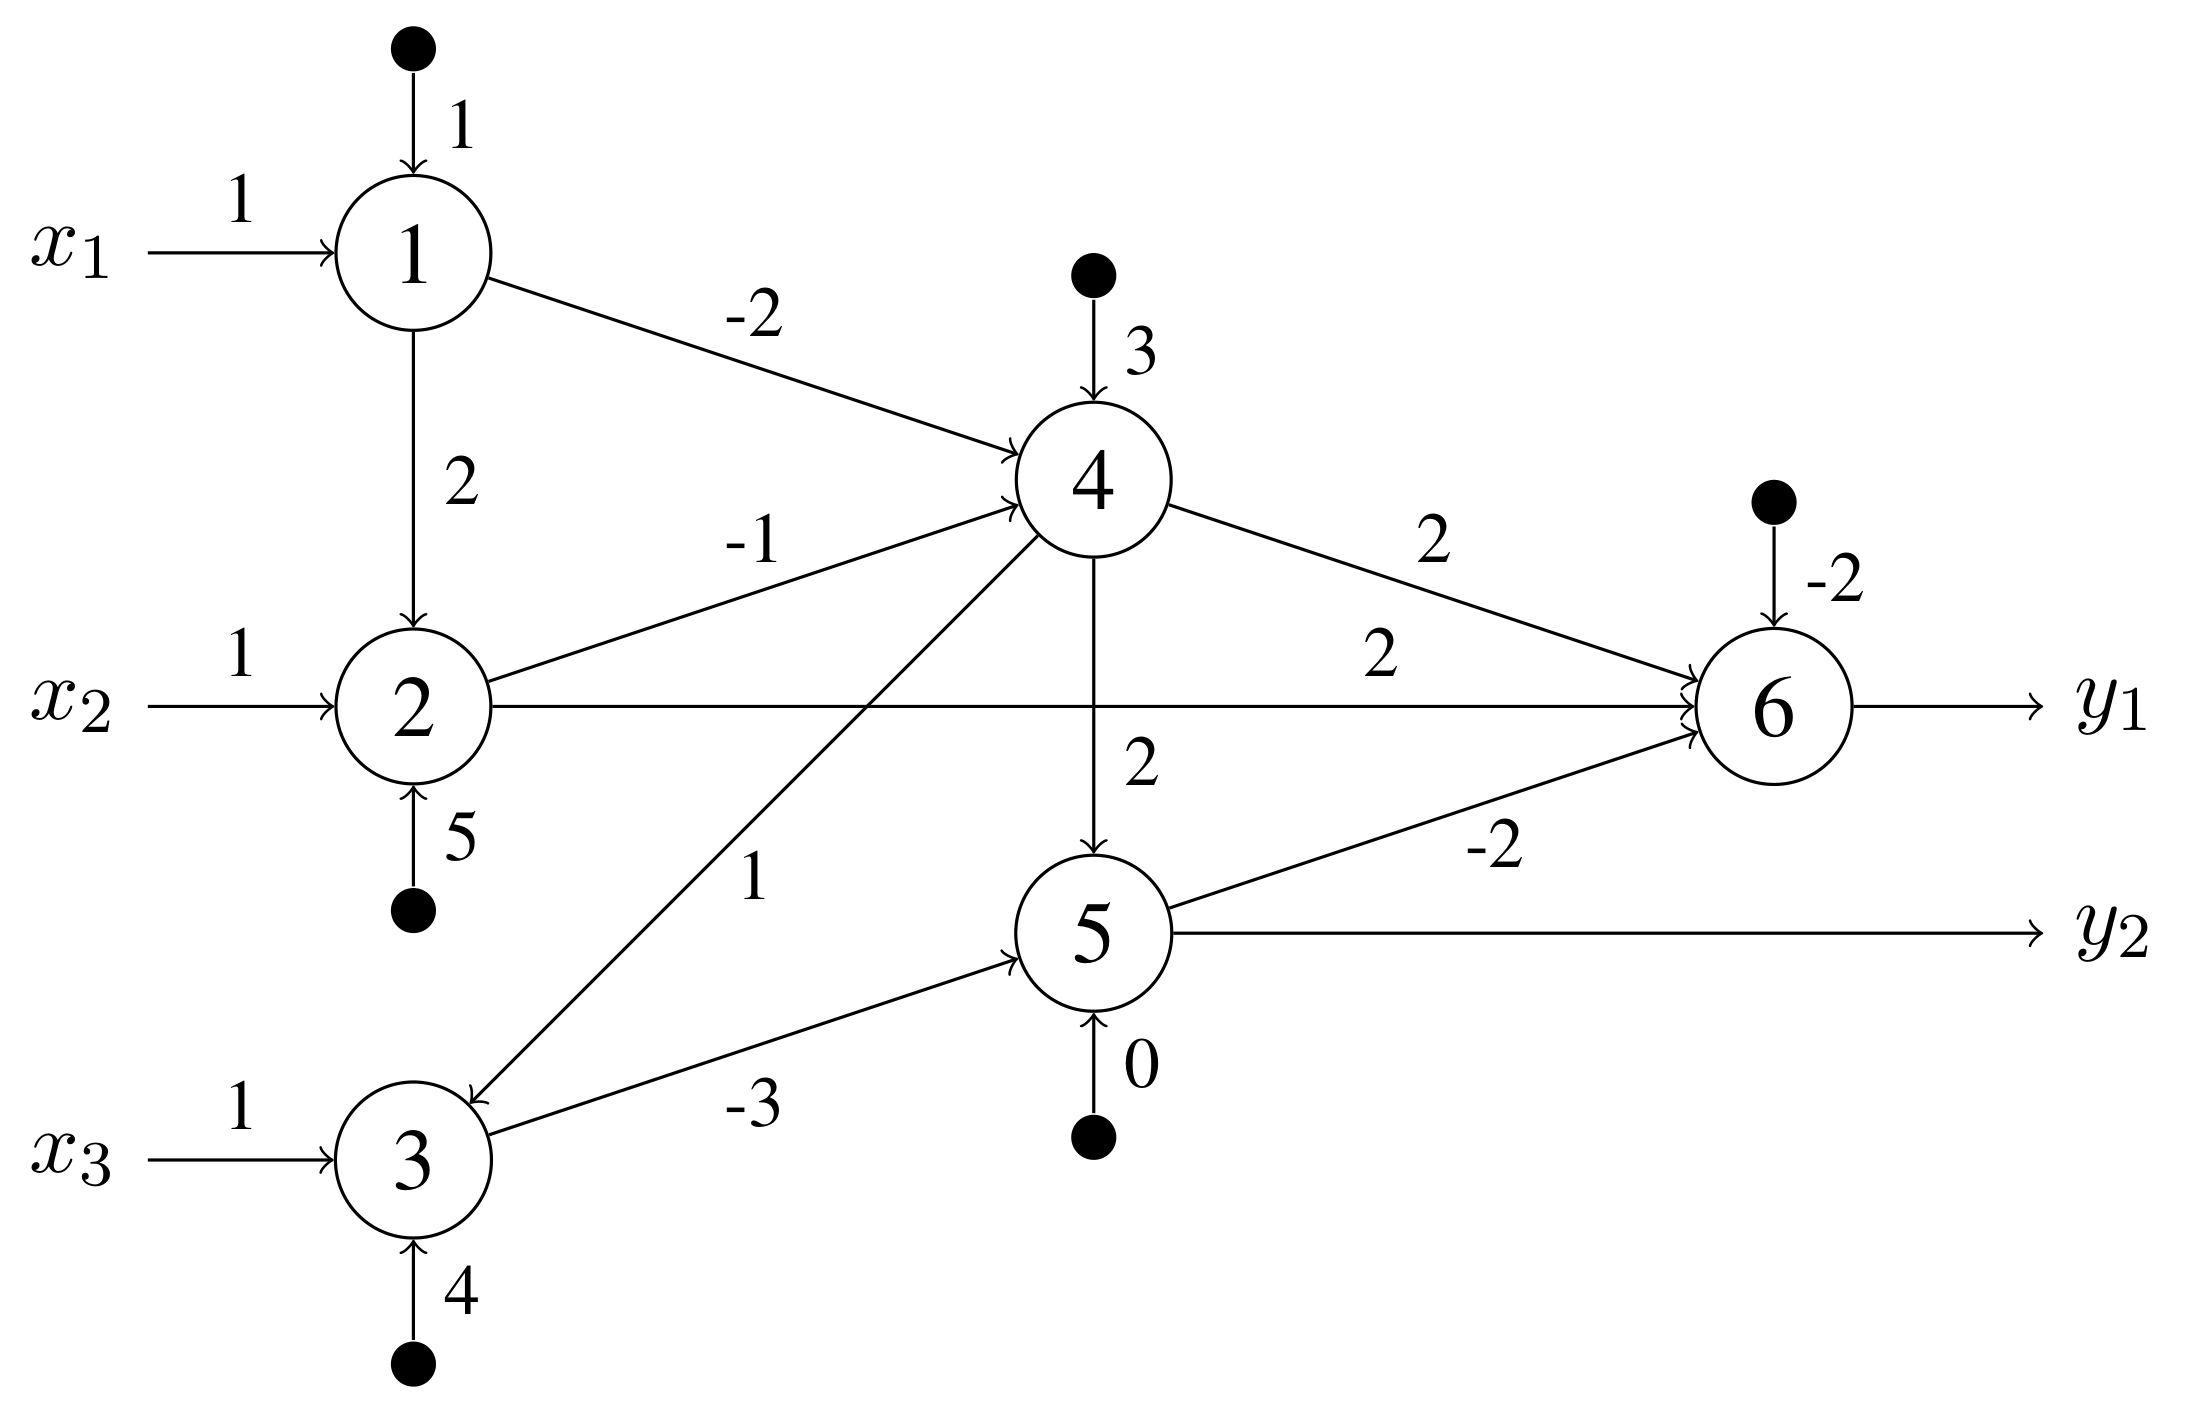
\includegraphics[scale=0.3]{neural_net.png}
    \end{figure}

    The numbers next to the arrows denote the respective weights. Nodes 1 and 4 have $g(x) = -x$ as their activation function. Node 3 uses the identity function $g(x) = x$. Nodes 2 and 6 use a hard limiter with a threshold of $0.5$, while node 5 uses the sigmoid function $g(x) = 1/(1 + e^{-x} )$.
    
    What is the output produced by the network when the input is $(x_1 ,x_2 ,x_3 ) = (1,0,1)$?

    \solution{}
\end{homeworkProblem}

\begin{homeworkProblem}
    Design a neural network with six binary input signals $S_0$, $S_1$, $I_0$, $I_1$, $I_2$, $I_3$ and a single binary output signal $I_{out}$ , which behaves as a 4-bit multiplexer. You are free to determine the structure of the network and the activation function yourself.

    As a reminder, a 4-bit multiplexer uses its select inputs ($S_0$ and $S_1$ ) to select and propagate one of the four input values. The remaining input values are ignored. The following truth table illustrates this behavior:

    \begin{table}[ht]
        \setlength\extrarowheight{-3pt}
        \centering
        \begin{tabular}{c|c|c|c|c|c||c}
            $S_1$ & $S_0$ & $I_0$ & $I_1$ & $I_2$ & $I_3$ & $I_{out}$ \\
            \hline \hline
            0 & 0 & 1 & * & * & * & 1\\
            0 & 0 & 0 & * & * & * & 0\\
            0 & 1 & * & 1 & * & * & 1\\
            0 & 1 & * & 0 & * & * & 0\\
            1 & 0 & * & * & 1 & * & 1\\
            1 & 0 & * & * & 0 & * & 0\\
            1 & 1 & * & * & * & 1 & 1\\
            1 & 1 & * & * & * & 0 & 0\\
        \end{tabular}
    \end{table}

    Note: \textit{The * symbol means that the signal at the given position can be either 1 or 0, as its value does not affect the output in any way.}

    \solution{}
\end{homeworkProblem}

\newpage

\begin{homeworkProblem}
    Consider a 2-layer perceptron with two input neurons and one output neuron of the following form:

    \begin{figure}[ht]
        \centering
        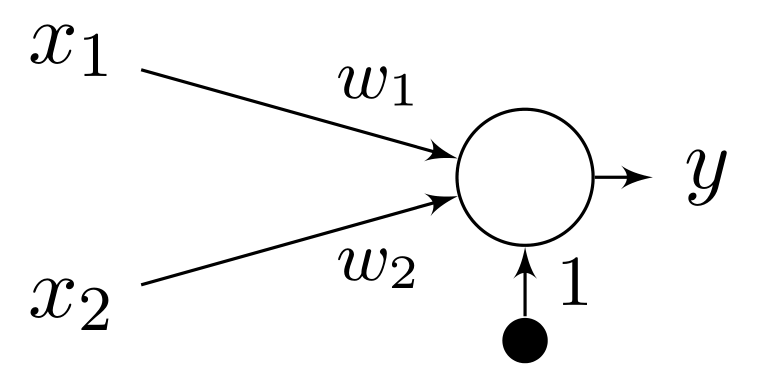
\includegraphics[scale=0.5]{2_layer_perceptron.png}
    \end{figure}

    Train the perceptron using the \textit{Perceptron learning rule} and the identity activation function ($g(x) = x$) on the following training data: $f(0,1) = 3, f(1,0) = 3$ and $f(1,1) = 5$. The weights are initialized to $0$ and the learning rate $\alpha$ is $1$. The bias weight will not be learned and stays $1$. Express algebraically the function $f(x_1 ,x_2)$ that your network has learned after the training is complete. Does this function produce the expected outputs for all three training inputs?
\end{homeworkProblem}

\begin{homeworkProblem}
    Use a single-layer perceptron with two inputs, one output and a bias weight, using the step function as activation function ($g(x) = 1$ for $x \geq t$ for some threshold $t$ and $g(x) = 0$ otherwise) to express the logical equivalence operator ($\equiv$) or provide a formal proof that no such construction is possible.

\end{homeworkProblem}
\end{document}
